%%-------------------------------------------------------------------------------------- Início
\begin{frame}[fragile,t]{Histórico}
  \begin{figure}[h!]
    \centering
    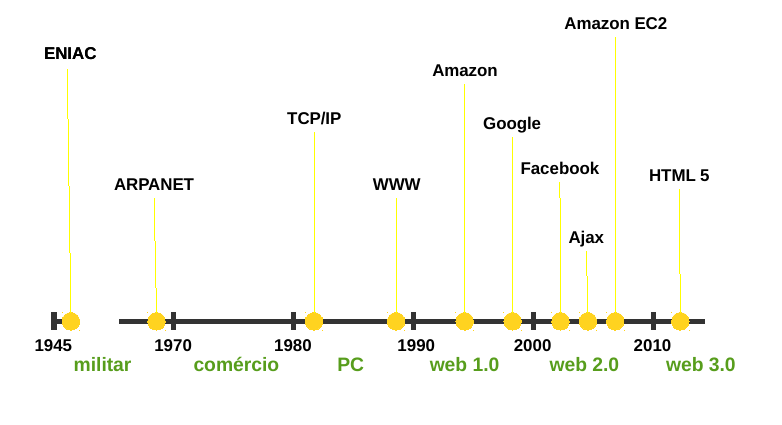
\includegraphics[width=0.95\textwidth]{imagens/historico.png}
  \end{figure} 
\end{frame}
%%-------------------------------------------------------------------------------------- Início
\begin{frame}[fragile,t]{Web 1.0, 2.0 e 3.0}
  \begin{itemize}
    \item \alert{Web 1.0} : páginas estáticas e primeiros modelos de negócios.
    \item \alert{Web 2.0} : interactividade(Ajax), redes sociais e comércio eletrônico.
    \item \alert{Web 3.0} : 'Web Inteligente', interpretação da informação auxiliada por máquina 
    \begin{itemize}
      \item exemplo: sistemas de recomendação.
    \end{itemize}
    \item Base \alert{tecnológica} da Web 2.0 e 3.0.
    \begin{itemize}
      \item javascript, xml, json(ajax).
      \item interoperabilidade via Web Services.
      \item infraestrutura via modelos de \alert{computação em nuvem} (IAAS, PAAS e SAAS)
      \item aplicações móveis
    \end{itemize}
  \end{itemize}
\end{frame}
%%-------------------------------------------------------------------------------------- Início
\begin{frame}[allowframebreaks, fragile,t]{Modelos de Computação em Nuvem}
  
  \begin{itemize}

    \item \alert{IAAS (Infraestructure As A Service)} : fornece a insfraestrutura computacional
      física ou máquinas virtuais e outros recursos discos, firewalls, endereços IP e etc.
    \begin{itemize}
     \item exemplos: Amazon EC2, Windows Azure, Google Compute Engine.
    \end{itemize}
    
    \item \alert{PAAS (Platform as a Service)} : fornece plataformas computacionais que tipicamente incluem sistemas operacionais,
      ambientes para execução de programas, bancos de dados, servidores web e etc.
    \begin{itemize}
     \item exemplos: AWS Elastic Beanstalk, Windows Azure, Heroku e Google App Engine
    \end{itemize}

    \item \alert{SAAS (Software as a Service)} : fornece acesso sob demanda às aplicações de software, sem que o usuário
      tem que se preocupar com sua instalação, configuração e execução.
    \begin{itemize}
     \item exemplos: Google Apps e Microsoft 365.
    \end{itemize}
 
  \end{itemize}
 
\end{frame}